\documentclass[../../main.tex]{subfiles}

\usepackage{gensymb}
\usepackage{textcomp}
\usepackage[colorlinks=true]{hyperref}

\begin{document}
\
\section{Sensor de Temperatura}

\subsection{Introducción}

Se implementará un sensor de temperatura utilizando el circuito integrado LM35, un circuito integrado cuya tensión de salida varía linealmente con la temperatura. \par
Según la datasheet del integrado mencionado anteriormente del fabricante Texas Instruments ''LM35 Precision Centigrade Temperature Sensors'', con última revisión en diciembre de 2017, el integrado ofrece un rango de medición asegurada de entre -55\celsius y 150\celsius, con una variación de 10mV/\celsius, siendo el 0\celsius correspondiente a 0V. \par
Se busca implementar a partir de estos valores, un sensor de temperatura capaz de medir con máxima excursión entre 35°C y 45°C, con 0V correspondiendo a 35\celsius y 5V a 45\celsius.\par
A partir del circuito se podrá utilizar un conversor analógico-digital para lograr manipular la información de temperatura como se requiera. \par
Se tuvo como prioridad minimizar la cantidad de componentes utilizados, garantizar la confiabilidad y precisión de los valores que el circuito devuelva. Se tuvo en cuenta la protección del circuito receptor de la señal, haciendo que la señal de salida no sobrepase el intervalo [-1;6] volts.

\subsection{Análisis del LM35 y condiciones a tener en cuenta}
\label{condiciones} 	%marker para link a esta seccion

Según la datasheet mencionada anteriormente, deben mencionarse ciertas consideraciones a tener en cuenta: 
\begin{itemize}
\item El error máximo del LM35 para medir temperatura es de 0.5\celsius, por lo que el circuito derivado a partir de él no podrá asegurar un error menor a este mismo.
\item La tensión de alimentación para el LM35 será de entre -0.2 V y 35 V como valores máximos, 4V  y 30 V como valores típicos.
\item La máxima temperatura de juntura es 150\celsius, la cual no se contradice con el rango de valores elegidos para el circuito implementado. La máxima temperatura de juntura es la máxima temperatura que la juntura del semiconductor interno puede tolerar manteniendo al LM35 en estado operativo.
\item La corriente de entrada del LM35 será baja, de 60$\mu$A máximo.
\item La corriente de salida del LM35 tomará un valor máximo de 10mA.
\item El LM35 tiene una impedancia de salida baja, de 0.1$\ohm$.
\end{itemize}

Es importante hacer notar que una baja impedancia de salida se corresponde con un circuito emisor de señal como es el caso de un sensor de temperatura. Esto es así porque si la señal emitida en tensión deberá ser recibida por otro circuito que interpretará o modificará la señal recibida, y si la impedancia de entrada del circuito receptor fuera más baja que la de salida del emisor, entonces
siendo z1 la impedancia de salida del emisor y z2 la impedancia de entrada del receptor, basándonos en el teorema de Thevenin, se realiza un divisor de tensión:
$V_o$ = $\frac{z_{2}}{z_{1}\text{+}z_{2}}$ $V_i$\par
Donde $V_i$ es la tensión de entrada y $V_o$ la de salida. Si se asume que la potencia se mantiene constante en el traspaso entre los dos circuitos, se aprecia de aquí que si |z1|«|z2| y 1«|z2|, entonces $\frac{z_{2}}{z_{1}\text{+}z_{2}}\approx 1$, con lo cual la tensión de salida del circuito emisor original sería equivalente a la tensión de entrada del circuito receptor, por lo que la señal sería recibida correctamente en valor. \par
Es por esto que se intentará obtener una impedancia de entrada de nuestro circuito adaptador mucho mayor a la impedancia de salida de 0.1$\ohm$ del LM35.

\subsection{Cambio de rango operacional}
\label{cambioRango} 	%marker para link a esta seccion
El comportamiento del LM35 puede ser representado matemáticamente con una transformación lineal de grados celsius a tensión en volts\par 
$TL_{35}$: c$\epsilon$ [-55; 150] -> v$\epsilon$[-0.55; 1.5] / $TL_{35}$(c) = 0.01$\cdot$c. 
El circuito a implementar pretende utilizar una transformación lineal\par
$TL_{cambio}$: $v_1\epsilon$ [0.35;0,45] -> $v_2\epsilon$ [0;5] de forma tal que 
$TL_{cambio}(TL_{35}(c))= TL_{sensor}(c)$ donde $TL_{sensor}: c\epsilon [0.35;0,45] -> v_2\epsilon[0;5]$ será la transformación total del circuito.

Así, se deberá resolver el siguiente sistema de ecuaciones:

	 \begin{equation}
  	   \left\{
	  	    \begin{array}{ll}
		 					0 = m\mathrm{\cdot}0.35 + b \\
			 				5 = m\mathrm{\cdot}0.45 + b \\
	     	 \end{array}
	     	\right.
 	\end{equation}

Que tiene como solución m=50 $\cap$ b = -17.5.

Para realizar la transformación lineal sobre la salida del LM35, se decidió utilizar un opamp con realimentación negativa, dispuesto de la siguiente manera:

\begin{figure}[H]	%y = mx +b en circuito
	\centering
	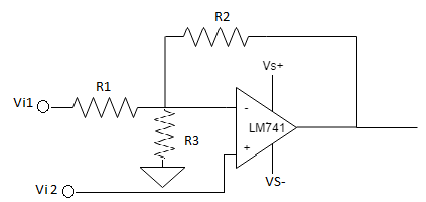
\includegraphics[scale=1.3]{imagenes/adder.png}
	\caption{Cambio de rango operacional en circuito}
	\label{fig:ej6_adder}
\end{figure}

El cual se resolverá por superposición (suponemos que el opamp está operando en su zona lineal) para mostrar que efectivamente realiza la transformación requerida:
\begin{itemize}
\item Pasivamos la fuente Vi1, dejando un no inversor:
\begin{figure}[H]	%vi1 pasivada
	\centering
	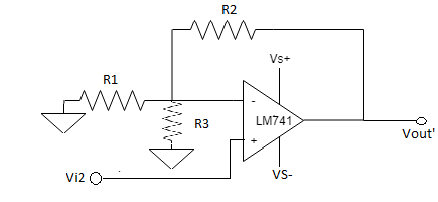
\includegraphics[scale=1.3]{imagenes/adder_pasivo_vi1.png}
	\caption{Vi1 pasivada}
	\label{fig:ej6_adder_pasivo_vi1}
\end{figure}
Entonces Vout' = $(1+\frac{R2(R1+R3)}{R1R3})\cdot$Vi2

\item Pasivamos la fuente Vi2, dejando un inversor:
\begin{figure}[H]	%vi2 pasivada
	\centering
	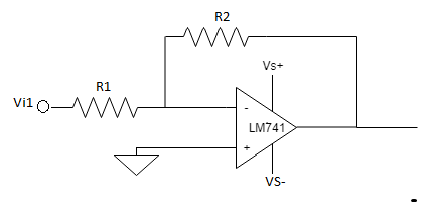
\includegraphics[scale=1.3]{imagenes/adder_pasivo_vi2.png}
	\caption{Vi2 pasivada}
	\label{fig:ej6_adder_pasivo_vi2}
\end{figure}

Entonces Vout'' = $-\frac{R2}{R1}\cdot$Vi1
\item Obtenemos la salida como la superposición de los dos estados calculados anteriormente:\par
Vout = Vout' + Vout'' = $(1+\frac{R2(R1+R3)}{R1R3})\cdot$Vi2 $-\frac{R2}{R1}\cdot$Vi1\par

Si Vi1 es una entrada continua positiva de valor Vs+ y Vi2 es la salida del LM35, entonces, para cumplir tanto con y = mx + b como con la solución al sistema de ecuaciones mencionada anteriormente: \par
	 \begin{equation}
  	   \left\{
	  	    \begin{array}{ll}
		 					50 = 1+\mathrm{\frac{R2(R1+R3)}{R1R3}}\\
			 				-17,5 = \mathrm{-\frac{R2}{R1}\cdot}Vs+ \\
	     	 \end{array}
	     	\right.
 	\end{equation}

 	
 	Por lo que si Vs+ es la alimentación del LM35 y, dado que el mismo se podrá alimentar con cualquier valor de tensión que caiga en el rango recomendado de entre $4V$ y $30V$, si se elige Vs+ = $7V$, \par

 El sistema queda definido como:
 		 \begin{equation}
  	   \left\{
	  	    \begin{array}{ll}
		 					\mathrm{R2} = \frac{35\, \mathrm{R1}}{2\, \mathrm{Vs+}} = \frac{5\, \cdot\mathrm{R1}}{2}\\
			 				\mathrm{R3} = \frac{5\, \mathrm{R1}}{14\, \mathrm{Vs+} - 5} = \frac{5\, \cdot\mathrm{R1}}{93}\\
	     	 \end{array}
	     	\right.
 	\end{equation}

\end{itemize}
\subsection{Protección del circuito a conectar}
\label{Protect}
Dado que el nuevo sensor a implementar será utilizado para alguna aplicación en concreto, deberá ser conectado a un segundo circuito ''receptor'' que utilice la información de la temperatura actual, por ejemplo un conversor analógico-digital. Es por esta razón que se prohibirán tensiones de salida que puedan resultar peligrosas para el receptor. Se garantiza que la salida, por ende, no será superior a 6V ni inferior a -1V. \par
Para lograr lo anterior, se utilizará un diodo Zener, que hará clipping asimétrico a la señal de salida (ver pedal de distorsión o ej5 para mayor información sobre clipping).\par
Los \underline{diodos Zener} suelen usarse para protección de circuitos y pueden ser representados por su curva característica:

\begin{figure}[H]	%curva diodo zener
	\centering
	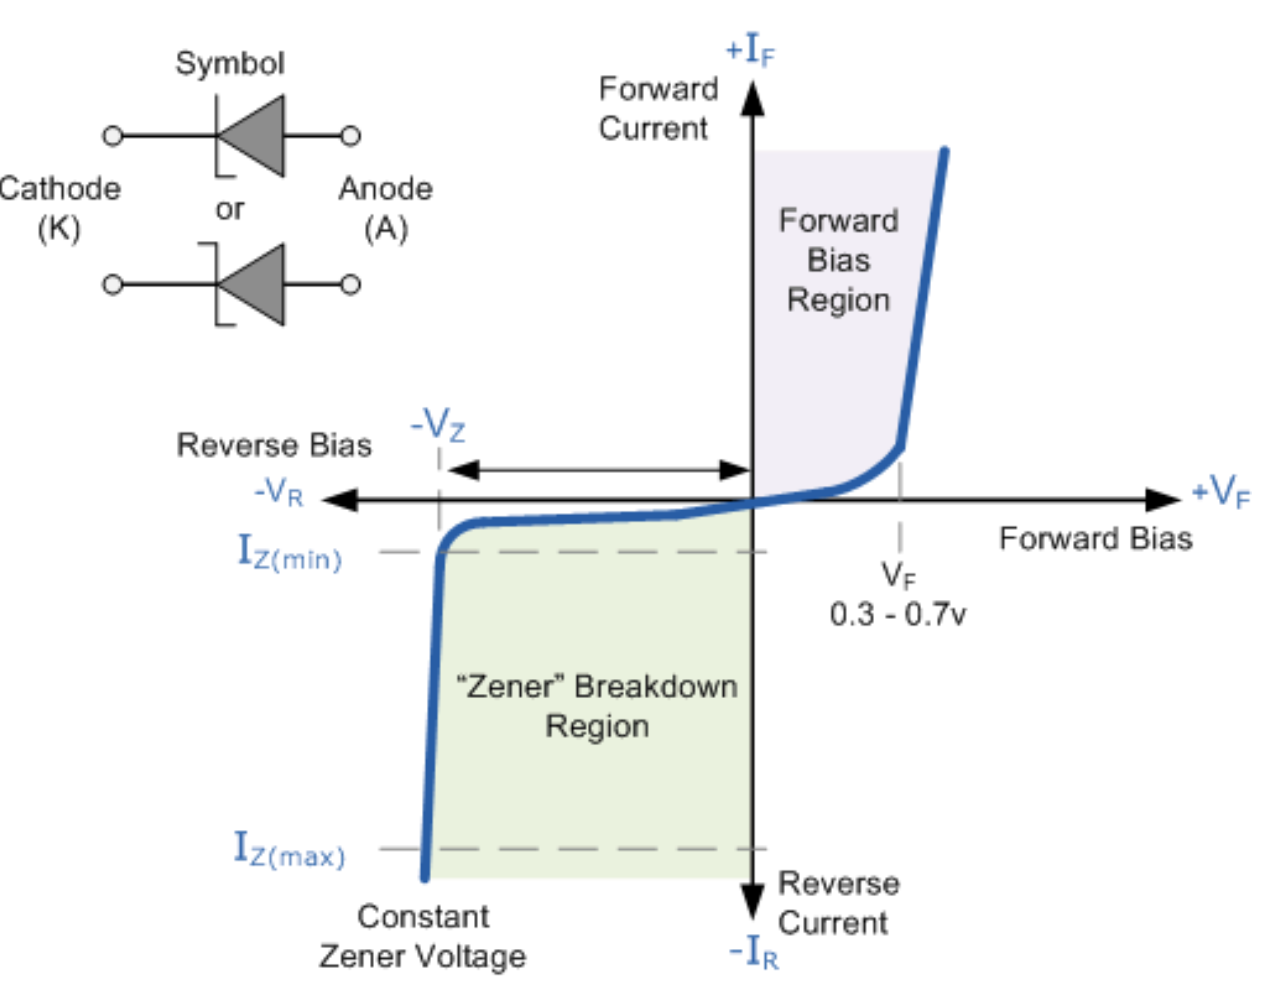
\includegraphics[scale=0.5]{imagenes/zener_diode_curva.png}
	\caption{Curva característica del diodo Zener}
	\label{fig:ej6_zener_diode_curva}
\end{figure}

De esta curva se hace notar que al superar el valor de tensión $V_f$ o al llegar a un nivel de tensión menor a $V_z$, la demanda de corriente por parte del diodo aumentará exponencialmente. Es aquí cuando recordamos una de las condiciones de la subsección \nameref{condiciones}: La corriente de salida del LM35 tomará un valor máximo de 10mA. Esto deberá ser tenido en cuenta cuando se presente la implementación final del circuito, junto con la salida de corriente máxima del opamp a utilizar para la transformación lineal.\par
De esta manera, se buscará que los valores de $V_f$ y $V_z$ sean tales que la demanda de corriente sea tan alta luego de los mismos que la tensión de salida no pueda estos valores para que se logre suplir. De esta manera, se muestra gráficamente la tensión de salida en función de la tensión de entrada:

\begin{figure}[H]	%curva diodo zener
	\centering
	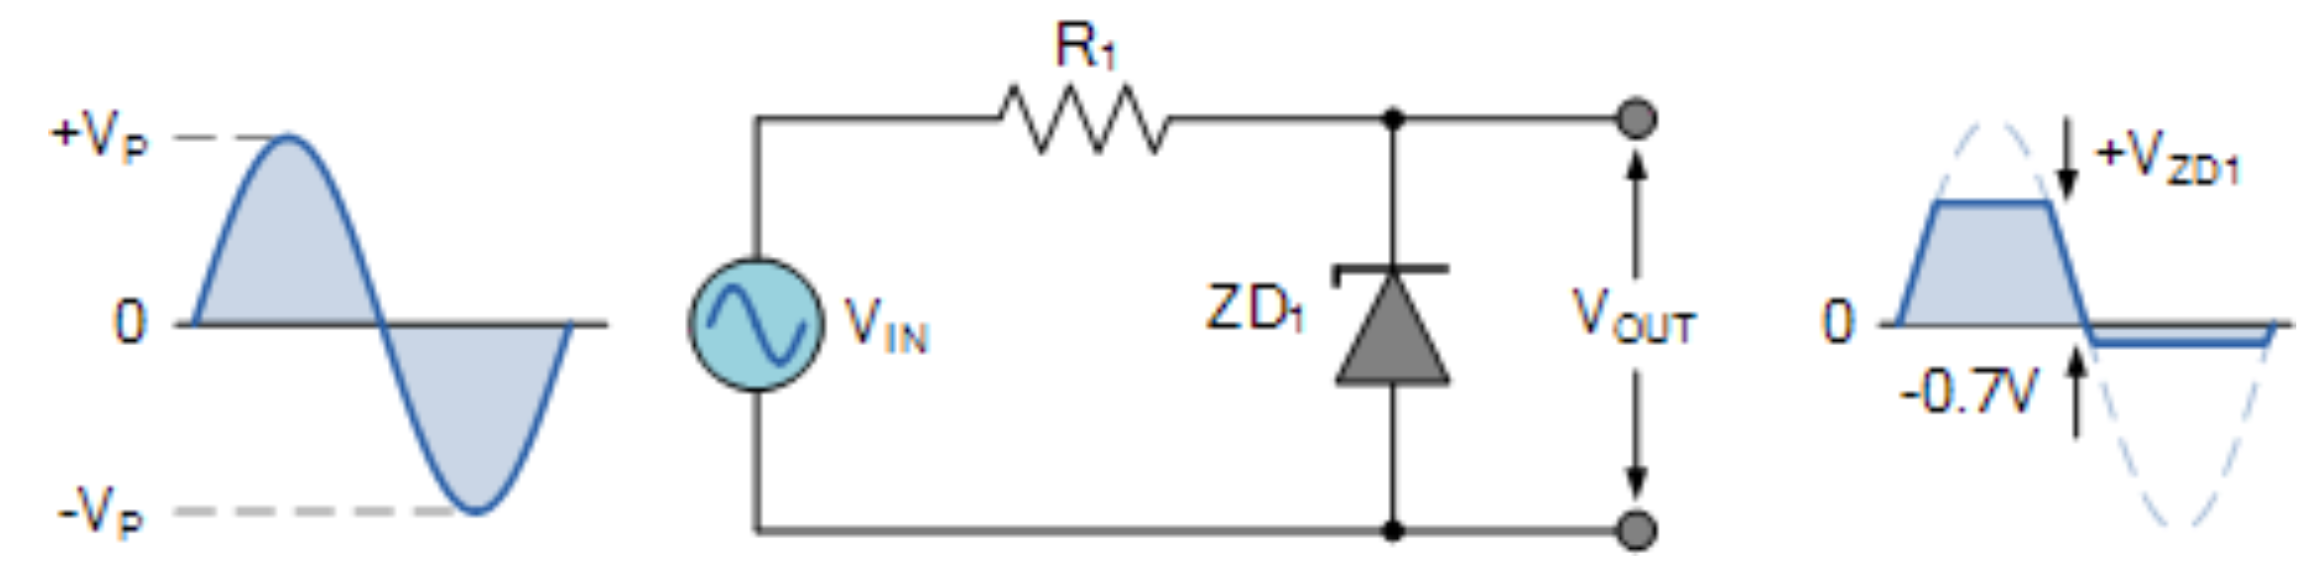
\includegraphics[scale=0.5]{imagenes/zener_diode_efecto.png}
	\caption{Efecto del diodo Zener sobre la entrada}
	\label{fig:ej6_zener_diode_efecto}
\end{figure}

Así es como se observa que $V_f$ = -0.7V y $V_z$$\approx$6V. Cabe destacar que el valor de $V_z$ es aproximado a 6V porque el valor no podrá ser excedido en absoluto como restricción de protección, por lo que $V_z<6V$. Se elige un valor $V_z= 5.6V$.

\subsection{Calibración del sensor}
\label{Calibration}
Debido al uso de fuentes no ideales y a los requerimientos de corriente de los opamps que generan ripple para la fuente, la tensión Vs+ de alimentación para el LM35 no necesariamente administrará el valor fijo de tensión antes designado de 7V, sino que será un valor cercano al anterior, y por lo tanto la relación entre resistencias mencionadas en la subsección \nameref{cambioRango} que se elija previamente a la implementación no será exacta. \par
Además, se sabe que los valores de resistencia nominales no necesariamente coinciden con los valores de resistencias reales de los componentes a la hora de realizar el circuito, y caerán dentro de un cierto rango centrado en su valor nominal definido por su tolerancia. \par
Es por esto que los valores de resistencias que se elijan de antemano no convergerán precisamente al offset y a la escala requeridas previamente (valores de m y b). De aquí que es necesario un proceso de calibración del sensor para su correcto funcionamiento.\par
El proceso de calibración, por ende, requerirá de ajustar los valores de resistencia de la subsección \nameref{cambioRango}. \par
Se observa que no se podrá ajustar los valores de offset y de escalamiento independientemente uno del otro, ya que si bien R3 solo participa del escalamiento, tanto R2 como R1 afectan al offset como así también al escalamiento, por lo que no se podrá alterar a R2 sin alterar al offset.\par
Es por esta razón que el método de calibración será necesariamente iterativo. Se obtiene así un método iterativo que converja al resultado esperado con el grado de error de calibración que requiera la persona que realice el ajuste. \par
Para lograr el calibrado y hacer R2 y R3 variables dentro de cierto rango, R2 y R3 ahora quedarán expresadas como la combinación de un potenciómetro y un valor fijo de resistencia en serie, de la siguiente manera:

\begin{figure}[H]	%R1 en función de un potenciómetro.
	\centering
	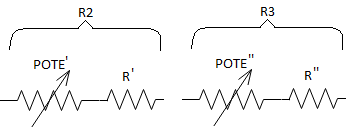
\includegraphics[scale=2]{imagenes/nueva_disposicion_rs.png}
	\caption{Expresión de R2 yR3 como combinación de potenciómetros en serie con resistencias fijas.}
	\label{fig:ej6_nueva_disposicion_rs}
\end{figure}

Una fuente externa se utilizará para calibrar el circuito, que simulará el input por parte del LM35. Se elige una fuente externa y no el LM35 para tener un rango de tensiones con el operar en vez de un único valor acorde a la temperatura actual determinada por el sensor. La señal a utilizar puede ser cualquiera que permita ajustar tanto la escala como la tensión de offset, pero se elige una rampa para la calibrar por su sencillez a la hora de determinar valor medio, amplitud y desplazamiento vertical.\par

\textbf{\underline{Método de calibración:}} 

Se conecta la salida del circuito a un osciloscopio.  
Se posiciona al switch de calibración en aquella posición que permite imponer una señal distinta a la del LM35 para calibrar. La fuente deberá generar una rampa (sawtooth signal) con duty cycle del 100\%, con LoLevel de 350mV y HiLevel de 450 mV. La frecuencia de esta señal deberá ser baja, eligiéndose a comodidad en un valor del orden de los 100 Hz. Se mide con el osciloscopio la señal de entrada, ajustando el trigger a comodidad.\par 

El método de calibración propuesto buscará lograr una suerte de cuasi-independencia entre R2 y R3. Se tratará a R2 como la resistencia que maneja al offset y R3 como la que manejará al escalamiento. Para el caso en el cual no se pueda seguir recurriendo a R2 para modificar al offset (es decir, el preset de R2 ha llegado a su límite), se podrá utilizar a R3 para acomodar a la señal. \par
Se seguirán los siguientes pasos:
\begin{enumerate}
	\item En el osciloscopio, se ajustará la escala vertical para lograr que se logren visualizar correctamente las dos señales. Tener en cuenta que la señal de salida estará finalmente situada entre los $0V$ y los $5V$, por lo que si se tiene que ajustar la escala en cualquier momento de la calibración, se deberá hacerlo.
	\item Se utilizará la base temporal del osciloscopio: La rampa de entrada y de salida se posicionarán de forma tal que las señales se corten en el extremo derecho de la pantalla y tengan su continuación en el extremo izquierdo de la pantalla sin saltos. Puesto de otra forma, se busca que el intervalo temporal del display de la señal sea un múltiplo natural del período de la señal. 
	\item Se pondrá en display el average de la señal usando las opciones de Quick Measure del osciloscopio. 
	\item Se modificará R2 (ajustando el preset) de manera tal que el valor medio o average de la señal de salida sea de $2.5V$. En el caso en que esto sea imposible porque se ha llegado al límite del preset, se podrá utilizar R3 para lograr que el valor medio o average de la señal de salida sea de $2.5V$.
	\item Se modificará R3 (ajustando el preset) de manera tal que o el extremo inferior de la señal de salida termine en 0V o el extremo superior termine en $5V$. Si no se puede seguir modificando a R3 porque se ha llegado al límite del preset, se da por terminado el paso.
	\item Si en el paso anterior tanto el extremo inferior coincide con los $0V$ y el superior con los $5V$, la calibración ha terminado. De lo contrario, se volverá al paso 4. 
	
\end{enumerate}

\subsection{Implementación del circuito}

\begin{figure}[H]	%circuito total
	\centering
	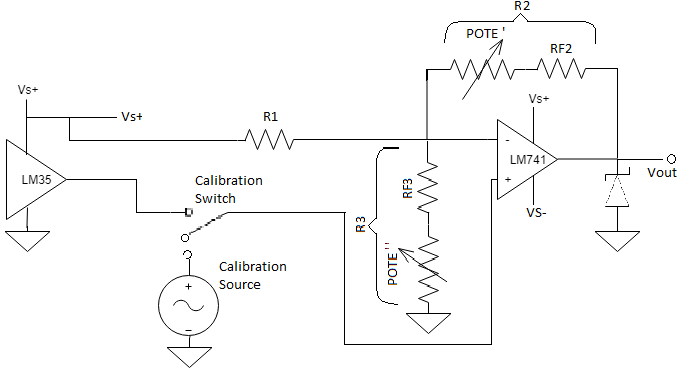
\includegraphics[scale=1.2]{imagenes/combinacion_circuito.png}
	\caption{Circuito propuesto como sensor}
	\label{fig:ej6_combinacion_circuito}
\end{figure}

Se hace notar que el switch físico que se utilizó es de tres posiciones en vez de dos porque el paniol no contaba con uno de dos. Además, deberá estar posicionado hacia el lado opuesto a la fuente de calibración para poder utilizarla, en el centro para apagar el circuito y en el otro extremo para utilizar al LM35 como input.
El diodo zener utilizado fue uno de Vz = 5.6 Volts, por lo que el circuito podrá devolver valores mayores a $5V$ y menores a $0V$ (pero que no salgan del intervalo de protección mencionado en la subsección \nameref{Protect}). Estos valores, que corresponderían a temperaturas fuera del intervalo [$0V$,$5V$], podrán ser interpretadas o filtradas por el conversor análogico digital que se utilice en conexión con el sensor de temperatura.
   
\subsection{Mediciones y conclusión}

Siguiendo los pasos del método de calibración de la sección \nameref{Calibration}, se logró ajustar al circuito:

\begin{figure}[H]	%circuito total
	\centering
	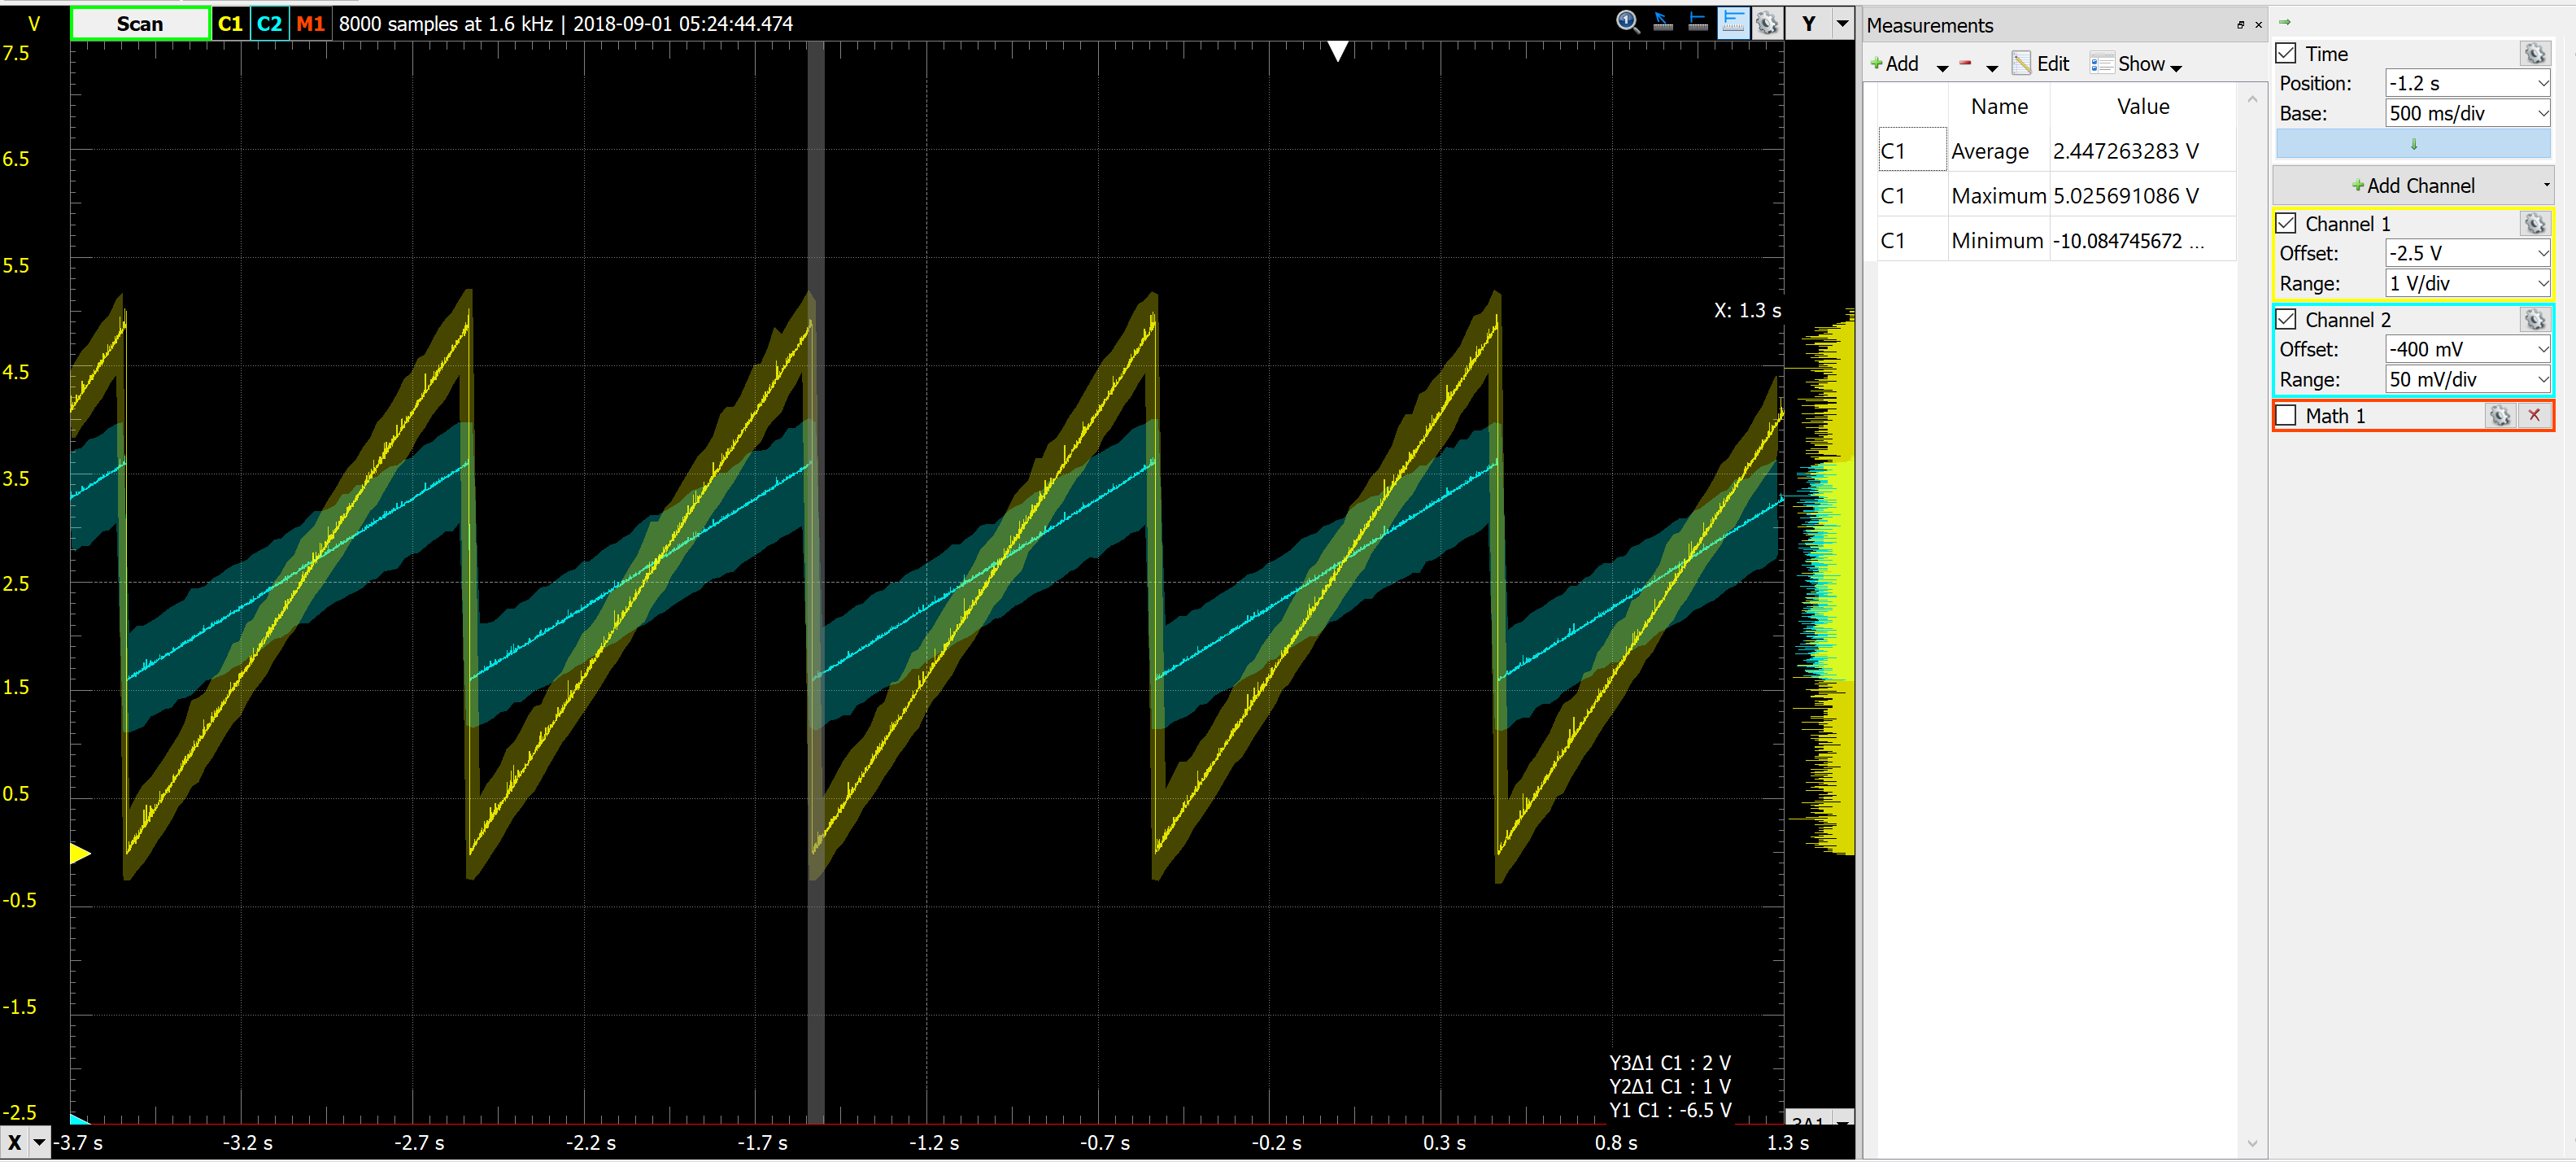
\includegraphics[scale=0.4]{imagenes/sensor_calibrado.png}
	\caption{Circuito calibrado. CH2:Entrada del circuito con la rampa de calibracion. CH1: Salida del circuito calibrado. }
	\label{fig:ej6_sensor_calibrado}
\end{figure}

De esta manera, se demuestra que el escalamiento y = 50 *x -17.5 se cumple con el circuito obtenido y el método de calibración es adecuado. \par
Se procedió a medir la temperatura con un tester del paniol y el LM35 con el osciloscopio y se verificó que las salidas coincidían.\par
Las ventajas del circuito implementado son predominantes en su bajo coste, ya que se utilizan pocas resistencias y un sólo integrado, en detrimento de la falta de independencia entre los presets y el factor que ajustan a la hora de calibrar. 
\end{document}
